\documentclass[oneside,numbers,spanish]{ezthesis}
%% # Opciones disponibles para el documento #
%%
%% Las opciones con un (*) son las opciones predeterminadas.
%%
%% Modo de compilar:
%%   draft            - borrador con marcas de fecha y sin im'agenes
%%   draftmarks       - borrador con marcas de fecha y con im'agenes
%%   final (*)        - version final de la tesis
%%
%% Tama'no de papel:
%%   letterpaper (*)  - tama'no carta (Am'erica)
%%   a4paper          - tama'no A4    (Europa)
%%
%% Formato de impresi'on:
%%   oneside          - hojas impresas por un solo lado
%%   twoside (*)      - hijas impresas por ambos lados
%%
%% Tama'no de letra:
%%   10pt, 11pt, o 12pt (*)
%%
%% Espaciado entre renglones:
%%   singlespace      - espacio sencillo
%%   onehalfspace (*) - espacio de 1.5
%%   doublespace      - a doble espacio
%%
%% Formato de las referencias bibliogr'aficas:
%%   numbers          - numeradas, p.e. [1]
%%   authoryear (*)   - por autor y a'no, p.e. (Newton, 1997)
%%
%% Opciones adicionales:
%%   spanish         - tesis escrita en espa'nol
%%
%% Desactivar opciones especiales:
%%   nobibtoc   - no incluir la bibiolgraf'ia en el 'Indice general
%%   nofancyhdr - no incluir "fancyhdr" para producir los encabezados
%%   nocolors   - no incluir "xcolor" para producir ligas con colores
%%   nographicx - no incluir "graphicx" para insertar gr'aficos
%%   nonatbib   - no incluir "natbib" para administrar la bibliograf'ia

%% Paquetes adicionales requeridos se pueden agregar tambi'en aqu'i.
%% Por ejemplo:
%\usepackage{subfig}
%\usepackage{multirow}

%% # Datos del documento #
%% Nota que los acentos se deben escribir: \'a, \'e, \'i, etc.
%% La letra n con tilde es: \~n.

\author{Percy Wilianson Lov\'on Ramos}
\title{Modelo para la localizaci\'on y seguimiento de un robot}
\degree{Ingeniero de Sistemas}
\supervisor{Por definir}
\institution{Universidad Nacional de San Agust\'in}
\faculty{Facultad de Ingenier\'ia de Producci\'on y Servicios}
\department{Escuela Profesional de Ingenier\'ia de Sistemas}

%% # M'argenes del documento #
%% 
%% Quitar el comentario en la siguiente linea para austar los m'argenes del
%% documento. Leer la documentaci'on de "geometry" para m'as informaci'on.

%\geometry{top=40mm,bottom=33mm,inner=40mm,outer=25mm}

%% El siguiente comando agrega ligas activas en el documento para las
%% referencias cruzadas y citas bibliogr'aficas. Tiene que ser *la 'ultima*
%% instrucci'on antes de \begin{document}.
\hyperlinking
\begin{document}

%% En esta secci'on se describe la estructura del documento de la tesis.
%% Consulta los reglamentos de tu universidad para determinar el orden
%% y la cantidad de secciones que debes de incluir.

%% # Portada de la tesis #
%% Mirar el archivo "titlepage.tex" para los detalles.
%% ## Construye tu propia portada ##
%% 
%% Una portada se conforma por una secuencia de "Blocks" que incluyen
%% piezas individuales de informaci'on. Un "Block" puede incluir, por
%% ejemplo, el t'itulo del documento, una im'agen (logotipo de la universidad),
%% el nombre del autor, nombre del supervisor, u cualquier otra pieza de
%% informaci'on.
%%
%% Cada "Block" aparece centrado horizontalmente en la p'agina y,
%% verticalmente, todos los "Blocks" se distruyen de manera uniforme 
%% a lo largo de p'agina.
%%
%% Nota tambi'en que, dentro de un mismo "Block" se pueden cortar
%% lineas usando el comando \\
%%
%% El tama'no del texto dentro de un "Block" se puede modificar usando uno de
%% los comandos:
%%   \small      \LARGE
%%   \large      \huge
%%   \Large      \Huge
%%
%% Y el tipo de letra se puede modificar usando:
%%   \bfseries - negritas
%%   \itshape  - it'alicas
%%   \scshape  - small caps
%%   \slshape  - slanted
%%   \sffamily - sans serif
%%
%% Para producir plantillas generales, la informaci'on que ha sido inclu'ida
%% en el archivo principal "tesis.tex" se puede accesar aqu'i usando:
%%   \insertauthor
%%   \inserttitle
%%   \insertsupervisor
%%   \insertinstitution
%%   \insertdegree
%%   \insertfaculty
%%   \insertdepartment
%%   \insertsubmitdate

\begin{titlepage}
  \TitleBlock{\scshape\insertinstitution}
  \TitleBlock[\bigskip]{\scshape\insertfaculty}
  \TitleBlock{\Huge\scshape\inserttitle}
  \TitleBlock{\scshape
    Tesis presentada por \insertauthor \\}
    %para obtener el grado de \insertdegree}
  \TitleBlock{\insertsubmitdate}
  \TitleBlock[\bigskip]{\insertdepartment}
\end{titlepage}

%% Nota 1:
%% Se puede agregar un escudo o logotipo en un "Block" como:
%%   \TitleBlock{\includegraphics[height=4cm]{escudo_uni}}
%% y teniendo un archivo "escudo_uni.pdf", "escudo_uni.png" o "escudo_uni.jpg"
%% en alg'un lugar donde LaTeX lo pueda encontrar.

%% Nota 2:
%% Normalmente, el espacio entre "Blocks" se extiende de modo que el
%% contenido se reparte uniformemente sobre toda la p'agina. Este
%% comportamiento se puede modificar para mantener fijo, por ejemplo, el
%% espacio entre un par de "Blocks". Escribiendo:
%%   \TitleBlock{Bloque 1}
%%   \TitleBlock[\bigskip]{Bloque2}
%% se deja un espacio "grande" y de tama~no fijo entre el bloque 1 y 2.
%% Adem'as de \bigskip est'an tambi'en \smallskip y \medskip. Si necesitas
%% aun m'as control puedes usar tambi'en, por ejemplo, \vspace*{2cm}.




%% # Prefacios #
%% Por cada prefacio (p.e. agradecimientos, resumen, etc.) crear
%% un nuevo archivo e incluirlo aqu'i.
%% Para m'as detalles y un ejemplo mirar el archivo "gracias.tex".
%%% Las secciones del "prefacio" inician con el comando \prefacesection{T'itulo}
%% Este tipo de secciones *no* van numeradas, pero s'i aparecen en el 'indice.
%%
%% Si quieres agregar una secci'on que no vaya n'umerada y que *tampoco*
%% aparesca en el 'indice, usa entonces el comando \chapter*{T'itulo}
%%
%% Recuerda que aqu'i ya puedes escribir acentos como: 'a, 'e, 'i, etc.
%% La letra n con tilde es: 'n.

\prefacesection{Agradecimientos}

Este trabajo no habr'ia sido posible sin el apoyo y el est'imulo de mi colega
y amigo, Doctor Rudolf Fliesning,  bajo cuya supervisi'on escog'i este tema y
comenc'e la tesis. Sr. Quentin Travers, mi consejero en las etapas finales
del trabajo, tambi'en ha sido generosamente servicial, y me ha ayudado de
numerosos modos, incluyendo el resumen del contenido de los documentos que
no estaban disponibles para mi examen, y en particular por permitirme leer, 
en cuanto estuvieron  disponibles, las copias de los  recientes extractos de
los diarios de campa'na del Vigilante Rupert Giles y la actual Cazadora la
se'norita Buffy Summers, que se encontraron con William the Bloody en 1998, y
por facilitarme el pleno acceso  a los diarios de anteriores Vigilantes
relevantes a la carrera de William the Bloody.

Tambi'en me gustar'ia agradecerle al Consejo la concesi'on de Wyndham-Pryce
como Compa'nero, el cual me ha apoyado durante mis dos a'nos de investigaci'on,
y la concesi'on de dos subvenciones de viajes, una para estudiar documentos
en los Archivos de Vigilantes sellados en Munich, y otra para la
investigaci'on en campa'na en Praga. Me gustar'ia agradecer a Sr. Travers,
otra vez, por facilitarme  la acreditaci'on  de seguridad para el trabajo en
los Archivos de Munich, y al Doctor Fliesning por su apoyo colegial y ayuda
en ambos viajes de investigaci'on.

No puedo terminar sin agradecer a mi familia, en cuyo est'imulo constante y
amor he confiado a lo largo de mis a'nos en la Academia. Estoy agradecida
tambi'en a los ejemplos de mis  difuntos hermano, Desmond Chalmers, Vigilante
en Entrenamiento, y padre, Albert Chalmers, Vigilante. Su coraje resuelto
y convicci'on siempre me inspirar'an, y espero seguir, a mi propio y peque'no
modo, la noble misi'on por la que dieron sus vidas. Es a ellos a quien dedico
este trabajo.

%% Por si alguien tiene curiosidad, este "simp'atico" agradecimiento est'a
%% tomado de la "Tesis de Lydia Chalmers" basada en el universo del programa
%% de televisi'on Buffy, la Cazadora de Vampiros.
%% http://www.buffy-cazavampiros.com/Spiketesis/tesis.inicio.htm


%% # 'Indices y listas de contenido #
%% Quitar los comentarios en las lineas siguientes para obtener listas de
%% figuras y cuadros/tablas.
\tableofcontents
%\listoffigures
%\listoftables

%% # Cap'itulos #
%% Por cada cap'itulo hay que crear un nuevo archivo e incluirlo aqu'i.
%% Mirar el archivo "intro.tex" para un ejemplo y recomendaciones para
%% escribir.
%% Los cap'itulos inician con \chapter{T'itulo}, estos aparecen numerados y
%% se incluyen en el 'indice general.
%%
%% Recuerda que aqu'i ya puedes escribir acentos como: 'a, 'e, 'i, etc.
%% La letra n con tilde es: 'n.

\chapter*{Resumen}
La presente investigaci\'on presenta un nuevo modelo basado en redes neuronales  para el seguimiento de un robot. El desempe\~no fue medido en funci\'on al error de la comparaci\'on entre la posici\'on estimada y la posici\'on real. Los resultados muestran una clara mejora de la localizaci\'on de objetos en ambiente multic\'amara frente a los m\'etodos tradicionales . El trabajo presentado tiene implicancias en los sistemas de visi\'on de f\'utbol de robots, casas inteligentes, vigilancia de ciudades, apoyo al control de velocidad vehicular.

%% Los cap'itulos inician con \chapter{T'itulo}, estos aparecen numerados y
%% se incluyen en el 'indice general.
%%
%% Recuerda que aqu'i ya puedes escribir acentos como: 'a, 'e, 'i, etc.
%% La letra n con tilde es: 'n.

\chapter*{Introducci'on}

A medida que la ciencia avanza, el desarrollo tecnol\'ogico tambi\'en lo hace; sobretodo en lo que implica facilitar y mejorar la calidad de vida del ser humano, es as\'i que los robots han tomado un papel importante en el cumplimiento de este prop\'osito. Los robots tienen diversas aplicaciones, siendo una de ellas la industria, en la cual se pretende ayudar en el proceso de fabricaci\'on de productos y/o servicios utilizando robots para tal cometido\cite{Morales_g}. Otra aplicaci\'on importante es la milicia, donde los robots tienen mayor repetitividad y precisi\'on \cite{Garcia_g}. Tambi\'en se tiene una creciente influencia en la agricultura, debido a la falta de mano de obra en tareas que hacen peligrar la integridad del ser humano \cite{Vasquez_g}.\\
Para que los robots no necesiten intervenci\'on de la  mano humana  en  su  interacci\'on    con el mundo exterior (autonom\'ia) es necesario que tengan sensores que sean eficientes. Una de las formas de sensoriamiento m\'as importantes es la de visi\'on. Baltes y Anderson mencionan que hay dos tipos de visi\'on, una que es la visi\'on local y la otra global. En la Visi\'on Local el robot tiene  una perspectiva de primera persona; en esta el robot tiene una c\'amara puesta sobre su propia estructura, este tipo trae ciertas dificultades como que el robot s\'olo puede ver lo que su campo de visi\'on le permite, adem\'as si el ambiente multirobot se requerir\'ia c\'amara para cada uno de los robots.  \cite {Baltes_g} \\
Por otro lado, la visi\'on global, es la que contiene una o mas c\'amaras (multic\'amara) las cuales cubren todo el espacio de trabajo, ser\'ia mejor llamada  espacio inteligente. Un espacio inteligente contiene \textit{sensores} los cuales tienen el rol de identificar los objetos y recibir informaci\'on del mundo exterior, \textit{procesadores} los cuales  son el n\'ucleo del proceso de vision ya que procesan la informaci\'on, \textit{actuadores}  y \textit{dispositivos de comunicacion} \cite{Brezac_g}.\\

El presente trabajo se probara la t\'ecnica de procesamiento de im\'agenes llamada Transformada de Hough y las redes neuronales  para realizar el seguimiento de un robot. \\

%% Los cap'itulos inician con \chapter{T'itulo}, estos aparecen numerados y
%% se incluyen en el 'indice general.
%%
%% Recuerda que aqu'i ya puedes escribir acentos como: 'a, 'e, 'i, etc.
%% La letra n con tilde es: 'n.

\chapter{Planteamiento y Justificaci\'on del Tema}
\section{Contexto y Motivaci\'on}
En el contexto de la visi\'on artificial, se tiene el tema de la visi\'on global cuyo  es la de detectar e identificar el objeto y  a partir de alli hacerle el seguimiento (Moving Object Tracking-MOT). Segun Achyara y Ray  se tienen dos enfoques para realizar el MOT: el enfoque basado en el reconocimiento y el basado en el movimiento. En el primero se estudia bajo las caracteristicas del objeto en el otro se usa las caracteristicas del movimiento del objeto \cite{acharya_g}.\\
El desafio se presenta cuando se utilizan c\'amaras de bajo costo y sin ning\'un estandar que permita su conexi\'on sencilla al computador.

\section{Definici\'on del Problema}
Un problema en la visi\'on global es el seguimiento de objetos, la aplicaci\'on en el tema de f\'utbol de robots ha sido explorada mediante sistemas de visi\'on que utilizan una sola c\'amara, sin embargo a\'un no se ha explorado con las t\'ecnicas que usaremos en la presente investigaci\'on.
\section{Objetivos}
\subsection{Objetivo General}
Verificar la utilizaci\'on de redes neuronales en el problema de localizaci\'on y seguimiento de un robot.
\subsection{Objetivos Espec\'ificos}
\begin{itemize}
\item Estudiar el estado del arte con respecto al tema.
\item Clasificar objetos est\'aticos de objetos en movimiento.
\item Adquisicion de secuencias de videos y procesamiento adecuado de ellas.
\item Dise\~no e implementaci\'on de un sistema que, basado en procesamiento de im\'agenes y redes neuronales permita realizar la trazabilidad del objeto(robot).
\item Probar el sistema propuesto, asi como entrenar la red neuronal recurrente que permita realizar la predicci\'on de posiciones sucesivas de un robot.
\end{itemize}

\section{Organizaci\'on de la tesis}
Se presenta una breve descripci\'on  de los contenidos en la presente tesis:
\subsection{Capitulo 2 Estado del Arte}
Se presenta un compendio de una gran parte de las investigaciones hechas en nuestro tema, tanto de fuentes no recientes (Rese\~na Hist\'orica ) y de las investigaciones mas recientes (Estado del Arte).
\subsection{Capitulo 3 Marco Te\'orico}
Se presenta un recorrido breve por la historia de la Rob\'otica, Redes neuronales, procesamiento de im\'agenes.
\subsection{Capitulo 4 Diagramas}
Se presentan los diagramas de casos de uso, diagrama de componentes y diagrama de clases, todos basados en el estandar UML.
\subsection{Capitulo 5 Propuesta}
Se presenta los componentes principales de la propuesta, se explica la forma en que se realiza el sistema de visi\'on y adem\'as el sistema de predicci\'on de las siguientes posiciones
\subsection{Capitulo 6 Evaluaci\'on}
Se presenta la puesta en practica de la propuesta asi como las comparaciones debidas entre lo que la propuesta predijo y las posiciones reales de los objetos.
\subsection{Capitulo 7 Conclusiones y Recomendaciones}
Se concluye con las conclusiones basadas en la experimentaci\'on realizada.
%% Los cap'itulos inician con \chapter{T'itulo}, estos aparecen numerados y
%% se incluyen en el 'indice general.
%%
%% Recuerda que aqu'i ya puedes escribir acentos como: 'a, 'e, 'i, etc.
%% La letra n con tilde es: 'n.

\chapter{Estado del Arte}
\section{Rese\~na Historica}
\subsection{\textbf{Sistemas de Visi\'on Global}}

Como ya mencionamos en la introducci\'on se prefiere el uso de sistemas globales para tener un panorama de todo el ambiente, este tipo de visi\'on nos evita la oclusion, pero sin embargo acarrea problemas como la sincronizaci\'on, si es que fuera en una sola computadora el problema de conectar varias c\'amaras es solucionado a veces c\'amaras de determinado est\'andar de dispositivos. Generalmente los sistemas de visi\'on global para los robots, se apoyan en marcas sobre los robots de forma de circulos los cuales les sirven  en el reconocimiento.\\
El problema de visi\'on global, tiene como uno sus focos principales el problema de la calibraci\'on de c\'amaras que permite establecer par\'ametros intr\'insecos y extr\'insecos (internos y externos) para que el funcionamiento de la camara sea correcto y no variable, dicho problema puede ser abordado con clustering por ejemplo el K-Means, en el que cada clase del algoritmo K-means es representado por un valor RGB(red,green,bluee) llamado centro  y se escoge aleatoriamente al inicio. Desp\'ues de tener los centros se podr\'ia agrupar  todos los que tienen centros m\'as cercanos, desp\'ues se saca la media y ese es el nuevo centro, el algoritmo terminaria cuando los centros ya no varian \cite{kelson_glo}.Este mismo enfoque nos puede servir para la segmentacion, esto dividiendo el conjunto de p\'ixeles y agruparlos segun su semejanza, ademas usar  de las redes neuronales para clasificar el color, en este caso tendriamos que darle a la red como valores de entrada los valores RGB de cada p\'ixel para que nos pueda retornar la identificaci\'on del color\cite{chabra_glo}.\\
El uso del color para obtener el reconocimiento del objeto deseado. Por ejemplo el sistema RoboRoos el cual es dividido en un total de 9 capas donde cada una tiene su tarea asignada. En este sistema se utiliza el color para diferenciar los diferentes objetos (robots, pelota), adem\'as se apoyan de c\'amaras que cumplen con el estandar IEEE Firewire, salvandose asi del problema de bus del USB cuando se trata de conectar varias c\'amaras\cite{ball_glo}. Adem\'as se puede aplicar el color usando mapas de color por ejemplo se puede realizar mapas de color para encontrar la crominancia (el componente que contiene informacion del color en cualquier video), despues de aplicar los mapas de color se verifica a traves de los contornos si es una pelota, o un jugador\cite{clau_glo}.
\\



\subsection{\textbf{Seguimiento de Objetos en Ambientes Multic\'amara}}
Si bien los sistemas de visi\'on globales nos proporcionan la ubicaci\'on, identificaci\'on de los objetos, es necesario hacerles un seguimiento, \'esto se hace por distintos m\'etodos que se tratar\'an en esta secci\'on. Esta tarea se puede realizar con una sola c\'amara pero no se puede cubrir todo el espacio bajo este enfoque, es por ello que se recomienda necesario implementar sistemas multic\'amara.\\

Uno de los enfoques que realizan los investigadores en el tema es el de la l\'ogica fuzzy el cual nos otorga un grado m\'as cercado a la percepcion humana, esto debido a las funciones de membres\'ia que nos indican grados de pertenencia  a los cuales puede pertenecer un color. Se pueden usar la l\'ogica fuzzy de diferentes formas por ejemplo utilizar aut\'omatas fuzzy donde cada estado de la aut\'omata $S_i$ representa en la c\'amara $i$ la aptitud para que sea esta c\'amara candidata a que en ella este el objeto que se sigue\cite{morioka_mul}, sin embargo este enfoque no es lo suficientemente robusto contra las oclusiones, ademas de solo realizar con una c\'amara. Tambien apoyados por un grafo de regi\'on de adayacencia para representar las imagenes del foreground, se pueden utilizar histogramas de color fuzificados asociados a cada regi\'on de adyacencia, los cuales combinados tienen bajo costo computacional y son aplicables en tiempo real\cite{hossiein_mul}.\\
Sin embargo existen otros enfoques relacionados tambi\'en  con el color como los que se basan en  histogramas de color, los cuales son fuertes contra el problema de oclusi\'on (los objetos tienden a confundirse mientras m\'as alejados estan de la c\'amara). Una forma es utilizando el coeficiente de Bhattachyara el cual apoya a la decisi\'on sobre cual c\'amara es la que tiene en su enfoque el objeto a seguir mediante un histograma \cite{nummiaro_mot}. Otra forma en la se puede hacer el seguimiento basado en histogramas es apoyarse del COBMAT (Color-Based Multiple Agent Tracking), este algoritmo nos permite distribuir el procesamiento del seguimiento de objetos, evitando asi la centralizaci\'on. Adem\'as de apoyarnos en c\'amaras inal\'ambricas\cite{oto_mul}.  \\
Algunos autores abordar el problema desde el punto de vista estoc\'astico,  en el cual es necesario a veces tener las probalidades a priori, \'esto se puede hacer un entrenamiento previo mediante una simulaci\'on de objeto para que el m\'etodo reconozca todo el espacio de trabajo utilizan una persona cargando una pelota y se reconoce la pelota, entonces desp\'ues de esto se puede utilizar una cadena de markov para dividir el espacio cubierto en una matriz de estados  y poder asi realizar el seguimiento\cite{Dick_mot}, sin embargo este enfoque tiene debilidades de cuando hay dos personas caminando en sentido contrario, se le puede confundir. \\
Adem\'as existen abordajes que se basan en las caracteristicas de determinados dispositivos y estandares para realiza el seguimiento.Por ejemplo las camaras Firewire, basadas Estandar IEEE 1394, el cual da facilidades para conectar varias c\'amaras, un problema vital para el enfoque de multic\'amaras\cite{kumar_mot}.\\
Un problema parecido al que se aborda en este paper, ser\'ia un enfoque distribuido en el que la comunicacion se realiza mediante el protocolo de comunicacion UDP(User Datagram Protocol), esto con el objetivo de seguir varios robots en ambiente multic\'amara, para facilitar el proceso de identificaci\'on del robot les ponen unas marcas con formas geom\'etricas(circulos). Utilizan dos tipos de enfoques para realizar la identificaci\'on uno es basado en el color y otro es basado en formas geometricas . Tienen dos programas diferentes, en uno es para controlar las c\'amaras y la adquisici\'on de im\'agenes y el otro programa es para centralizar la informaci\'on obtenida de las c\'amaras \cite{garcia_mot}. \\

\section{Estado del Arte}
Los estudios m\'as recientes en seguimiento objetos en ambientes multic\'amaras nos muestran diferentes m\'etodos como son los planos homogr\'aficos cuya principal caracter\'istica es que ahorran costo computacional. Santos y Thiago llegan a la conclusi\'on que algunos de los anteriores m\'etodos enfrentan problemas como la oclusi\'on y la confusion por colores cuando se tratan de objetos homogeneos. Ellos abordan de diferente forma ya que primero realizan la localizaci\'on, luego hacen una segmentaci\'on(\textit{locate-then-segment}), en contraste con los m\'etodos tradicionales que realizan primero la segmentaci\'on(\textit{segment-then-locate}). Adem\'as integran la informaci\'on de todas las c\'amaras antes de tomar una decisi\'on, la homograf\'ia la usan para fusionar la informaci\'on de el \textit{foreground} para resolver oclusiones y localizar en este caso personas en planos referenciales\cite{Santos_art}.Yaldaz adem\'as de  utilizar la homograf\'ia aumentan a ello  los llamados \textit{Voting Methods} los cuales les otorgan la facilidad de hacerlos paralelizables, no son iterativos y mas r\'apidos \cite{yaldaz_mot}. \\
Otra forma actual de abordar el problema de seguimiento es haciendo una representaci\'on en en grafos basada en las diferentes vistas de la camara.Hofmman utiliza un solo hipergrafo para realizar con el cual resuelve el problema de asociaci\'on de data, ademas su enfoque sirve para ambientes multic\'amara en las cuales hay sobreposici\'on de las vistas de las c\'amaras. Cada nodo de el hipergrafo contiene los acoplamientos factibles entre las c\'amaras para asegurarse que cada deteccion es en la misma direcci\'on (para ambas c\'amaras), esto nos hace se\~nalar que usan unas restricciones de acoplamiento. El problema de seguimiento lo abordan como un problema de m\'aximos globales a posteriori, cada detecci\'on es definida como una tupla en la que componen la posici\'on el tama\~no del pixel, el \'indice de la c\'amara, y el tiempo \cite{Hofman_art}.Leal aplica un grafo para cada posible vista de las c\'amaras, y si es necesario para cada tupla de camara\cite{Leal_art}\\
Tambien se pueden usar sistemas de visi\'on ya realizados por ejemplo el sistema de Visi\'on Anafocus Eye-RIS con un algoritmo  que combina la detecci\'on de objetos en movimiento con la extracci\'on de caracter\'isticas, el Eye-Ris utiliza el sensor de imagen inteligente \textit{(SIS)Anafocus} \cite{karabiber_mot}.\\
El problema tambien se esta abordando haciendo una representaci\'on en 3D dinamica bas\'andose en las vistas de cada c\'amara sin embargo se enfrentan 3 problemas principalmente: (1) Costo y complejidad computacional, (2) como cargar la representaci\'on hallada, (3) Los m\'etodos son muy generales y las aplicaciones muchas. Bilir hace una malla para hacer la representaci\'on inicial y la va cambiando segun el tiempo, liber\'andose as\'i del problema de tener representacion (mallas) ya predeterminadas para hacer la reconstrucci\'on. Utilizan el m\'etodo \textit{Shape Tracking} el cual trata de hacer una reconstrucci\'on de una superficie en el tiempo \emph{t+1} en funci\'on a la representaci\'on hallada en \emph{t}. Ellos realizan el seguimiento tomando atenci\'on a los cambios de la conectividad y dezplazamientos   de los vertices. Con este enfoque se puede recibir cualquier forma haciendo este enfoque mas din\'amico.\cite{Bilir_art}\\
Un abordaje que se realizo es el de usar el \textit{background} y el \textit{foreground} \'esto para saber cual es el objeto de fondo y el objeto en movimiento esto nos da la facilidad de evitar la oclusi\'on y las ambiguedades de apariencia, sin embargo esto necesita intervenci\'on del usuario para poder asistir al programa. Sin embargo se puede realizar un enfoque que no necesita de la intervenci\'on del usuario. Emplean \textit{Confidence Maps} que son calculados a trav\'es de la fusion de \textit{Foregrounds}, cada mapa es calculado para cada una de las vistas de las camaras, esto consiste en puntajes que representan la acumulativa confidencia en el ambiente multic\'amara si el pixel es \textit{foreground} o no lo es . Varias camaras estan de acuerdo que un punto especifico es parte del \textit{foreground}, adem\'as utilizan \textit{Particle Swarm Optimization } para optimizar la funcion de ajuste, este algoritmo sugiere que pixeles pertenecen al foreground y que parametros m\'as se pueden incluir para descartar los p\'ixeles que no los son, siendo asi un algoritmo que no necesita intervencion del usuario\cite {Greek_art}.
%% Los cap'itulos inician con \chapter{T'itulo}, estos aparecen numerados y
%% se incluyen en el 'indice general.
%%
%% Recuerda que aqu'i ya puedes escribir acentos como: 'a, 'e, 'i, etc.
%% La letra n con tilde es: 'n.

\chapter{Marco Te\'orico}
\section{Rob\'otica}
\subsection{Breve recorrido por la historia de la Rob\'otica}
La Rob\'otica fu\'e un t\'ermino acu\~nado por Isaac Asimov, el cual fue un escritor en su tiempo de ciencia ficci\'on, realidad en nuestra era. La rob\'otica tuvo sus inicios en la cultura griega, los cuales llamaban \emph{automatos} que era la palabra que ten\'ian para denominar a sus m\'aquinas, de esta palabra deriva \emph{automata}.\\
Los \'arabes (siglo VII a XV) utilizaron los conocimientos griegos para realizar m\'aquinas que ya no solo las usaban para su diversi\'on sino que comenzaron a darle aplicaciones pr\'acticas un ejemplo de ello eran los dispensadores de agua autom\'aticos. \\
Durante los siglos XVII y XVIII  se crearon algunas m\'aquinas con forma similar a los humanos y algunos animales, estos dispositivos creados en la mayor\'ia por el gremio de relojeros se utilizaban para la diversion y entretenimiento. \\
A finales del siglo VIII y principios del XIX se crearon algunas invenciones mec\'anicas como la hiladora giratoria de Hargreaves(1770), el telar mec\'anico de Cartwright (1785) y el telar de Jacquard (1801).\\
En 1948 R.C. Goertz del \emph{Argonne National Laboratory} desarrollo, el primer telemanipulador con el objetivo de manipular los elementos reactivos sin riesgo a los operadores humanos, este es el antecedente m\'as cercano a los robots, desp\'ues estos telemanipuladores evolucionaron y luego ya se hablaba de robots, cuyas primeras configuraciones eran como de esferas y antropom\'orficas. En 1982 El profesor Makino de la Universidad Yamanashi de Japon desarrolla el robot SCARA (\emph{Selective Compliance Assembly Robot Arm}) cuyo principal objetivo era el de ensabamblado de piezas en cadenas de produccion industriales. \cite{lib_rob1}.\\
En la Tabla a continuaci\'on podemos ver una breve linea del tiempo de los sistemas llamados Automatas durante el tiempo, anteriormente citados.\\\\


\begin{tabular}{|c|l|l|}
\hline 
\textbf{A\~no} & \textbf{Auto}r & \textbf{Aut\'omata} \\ 
\hline 
1352 & Desconocido & Gallo de la catedral de Estrasburgo \\ 
\hline 
1499 & L.Da Vinci & Le\'on Mec\'anico \\ 
\hline 
1525 & J. Turriano & Hombre de Palo \\ 
\hline 
1738 & J de Vaucanson & Flautista, tamborillero, pato \\ 
\hline 
1769 & W. Von Kempelen & Jugador de Ajedrez \\ 
\hline 
1770 & Familia Droz & Escriba, organista, dibujante \\ 
\hline 
1805 & H.Maillardet & Mu\~neca mecanica dibujante \\ 
\hline 
\end{tabular}
\subsection{Definicion de Rob\'otica y Sistema Rob\'otico}
La definicion de rob\'otica es la ciencia de estudio de la conexi\'on inteligente entre la percepcion y accion. Com\'unmente un sistema rob\'otico es un sistema complejo compuesto por m\'ultiples subsistemas (Fig 3.1). \\
La capacidad de un robot para poder ejecutar una accion viene dada por el \textit{Sistema de Actuadores} el cual anima los componentes mec\'anicos del robot. La capacidad de percibir el mundo exterior esta dado por el \textit{Sistema de Sensores} el cual modifica el estado interior del sistema mecanico tomando datos del mundo exterior. La capacidad de conectar la accion con la percepci\'on viene dada por el \textit{Sistema de Control} el cual ejecuta comandos siguiendo las reglas de la tecnica de planificaci\'on del robot.\cite{lib_rob2}
\begin{figure}
\centering
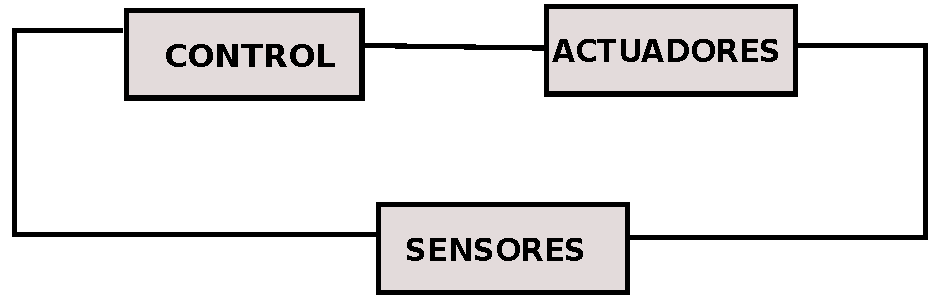
\includegraphics[width=3.0in]{imagen3.pdf}
\caption{Subsistemas dentro de un robot (Fuente: Elaboraci\'on Propia)}
\label{fig_mar}
\end{figure}

%%%%%%%%%%%%%%% ACA PUEDE IR ESA TABLA DEL LIBRO
 \section{Redes Neuronales}
 Las redes neuronales artificiales son estructuras paralelas las cuales se acercan al comportamiento de las redes neuronales humanas. Estan compuestas por neuronas  interconectadas mediantes axones donde varias neuronas pueden formar una capa (si se tratara de una red neuronal multicapa), y varias capas formar una neurona.\\
 Podemos explicar una red neuronal con salida binaria en la figura 3.2:\\
 
 \begin{figure}
\centering
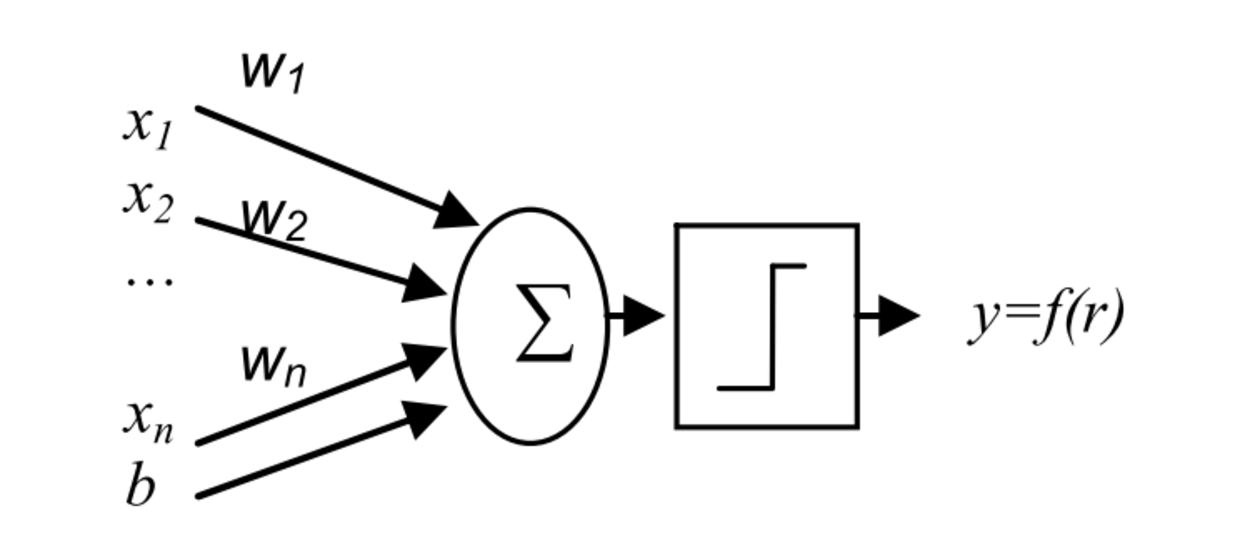
\includegraphics[width=3.0in]{imagen4.pdf}

\caption{Red Neuronal de Salida Binaria}
\label{fig_mar}
\end{figure}
Donde $x_1,x_2,x_3,...,x_n$ son las entradas para la red neuronal,$w_1,w_2,w_3,...,w_n$  son los pesos sinapticos, y $b$ es un factor de polarizaci\'on. El resultado final de la funci\'on se calcular asi: 
\begin{equation}
r= \sum_{i=1}^{n}x_iw_i+b
\end{equation}
El resultado de esta ecuaci\'on  nos dar\'a 1 o 0 y si se tratara de una red multicapa este seria la entrada para otra red neuronal.\cite{art_red1}

 \section{Procesamiento de Im\'agenes}
El procesamiento de im\'agenes es utilizado para mejorar las imagenes,prepararlas correctamente para un an\'alisis por parte de m\'aquinas. Consta de 4 procesos basicamente.\cite{art_red1}
\begin{enumerate}
\item Preprocesamiento: Son operaciones para adaptar la informaci\'on de una imagen y tenerla lista para el siguiente paso. Por ejemplo cambiar el brillo, reducir ruido.
\item Segmentacion: Separar la imagen en partes de las cuales se pueda hacer un analisis independiente.
\item Deteccion de objetos y clasificacion: Determinar cual objetos es cual.
\item Analisis de Imagen Obtener Informacion de alto nivel acerca de la imagen.
\end{enumerate}
 \begin{figure}
	\centering
	
\includegraphics[width=3.0in]{imagen5.pdf}
	\caption{Pasos del Procesamiento de Im\'agenes(Fuente: elaboraci\'on propia)}
	
	%%\label{fig_mar}
\end{figure}
% \subsection{Vision Artificial}
 %\subsection{Seguimiento de Objetos}
%%% Los cap'itulos inician con \chapter{T'itulo}, estos aparecen numerados y
%% se incluyen en el 'indice general.
%%
%% Recuerda que aqu'i ya puedes escribir acentos como: 'a, 'e, 'i, etc.
%% La letra n con tilde es: 'n.
%
%\chapter{Diagramas}
%\section{Diagrama de Casos de Uso}
%\begin{figure}
%	\centering
%	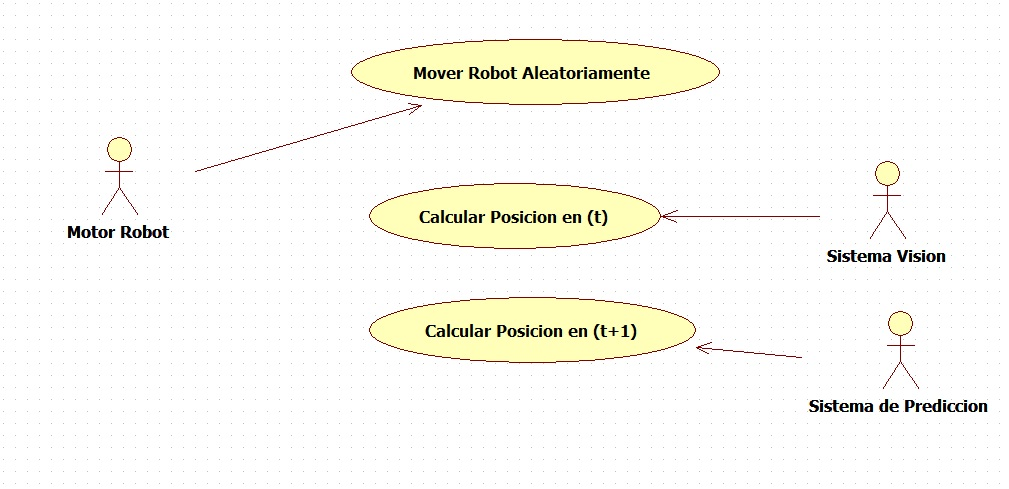
\includegraphics[width=4.5in]{imagen9.jpg}
%	
%	\caption{Diagrama de Casos de Uso}
%	\label{fig_mar}
%\end{figure}
%\section{Diagrama de Componentes}
%\begin{figure}
%	\centering
%	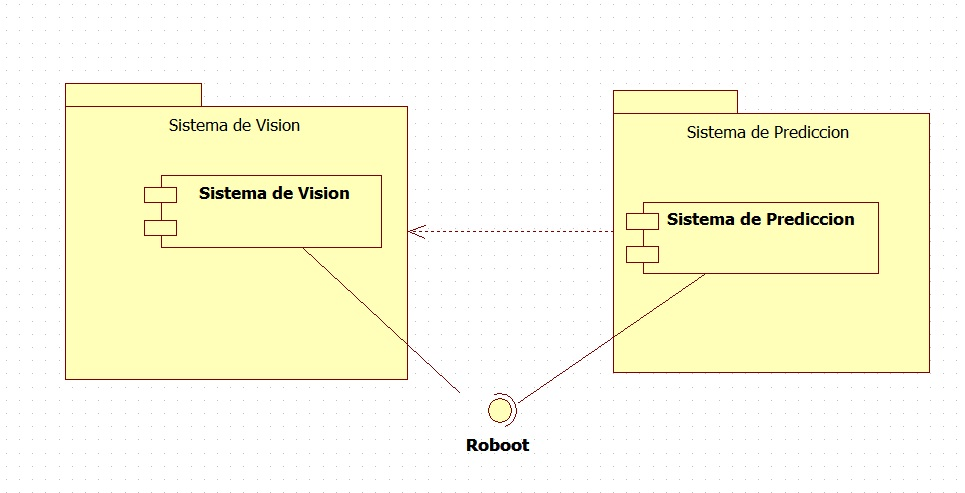
\includegraphics[width=4.5in]{imagen10.jpg}
%	
%	\caption{Diagrama de Componentes}
%	\label{fig_mar}
%\end{figure}
%
%
%\section{Diagrama de Clases}
%\begin{figure}
%	\centering
%	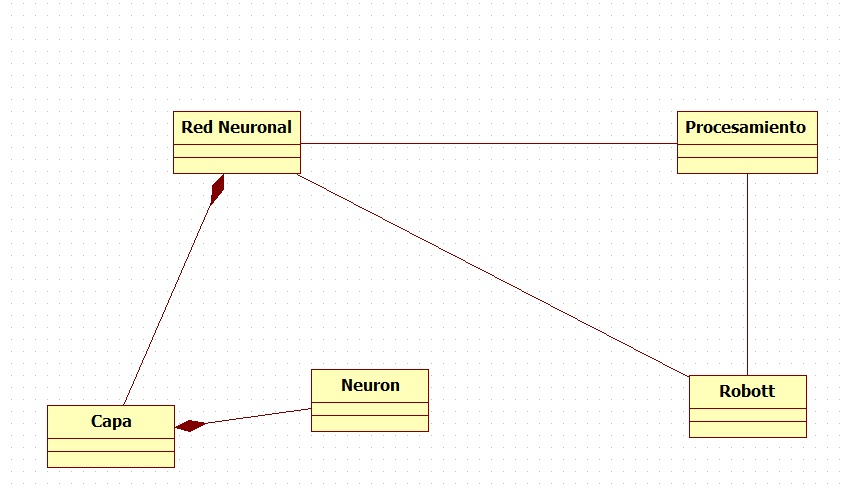
\includegraphics[width=4.5in]{imagen11.jpg}
%	
%	\caption{Diagrama de Clases}
%	\label{fig_mar}
%\end{figure}
%% Los cap'itulos inician con \chapter{T'itulo}, estos aparecen numerados y
%% se incluyen en el 'indice general.
%%
%% Recuerda que aqu'i ya puedes escribir acentos como: 'a, 'e, 'i, etc.
%% La letra n con tilde es: 'n.

\chapter{Propuesta}
Se propone un abordaje basado en la t\'ecnicas de procesamiento de imagenes que servir\'an para implementar el sistema de visi\'on global, el cual tendr\'a como salida la posici\'on y orientaci\'on actual en cada frame del robot. Luego de este proceso se utilizar\'a una red neuronal  que aprender\'a de los estados y las posiciones y predecir\'a los siguientes estados para hacerle el seguimiento. El esquema se presenta en la figura 4.1: \\
	\begin{figure}
	\centering
	
\includegraphics[width=2.5in]{esquema.pdf}
	
	\caption{Esquema del Sistema}
	\label{fig_mar}
\end{figure}
\section{Sistema de Visi\'on}
Para esto utilizamos marcas encima de los robots, las cuales nos dan mas facilidades para realizar la identificaci\'on de cada robot como se muestra en la Figura 4.2.
	\begin{figure}
	\centering
	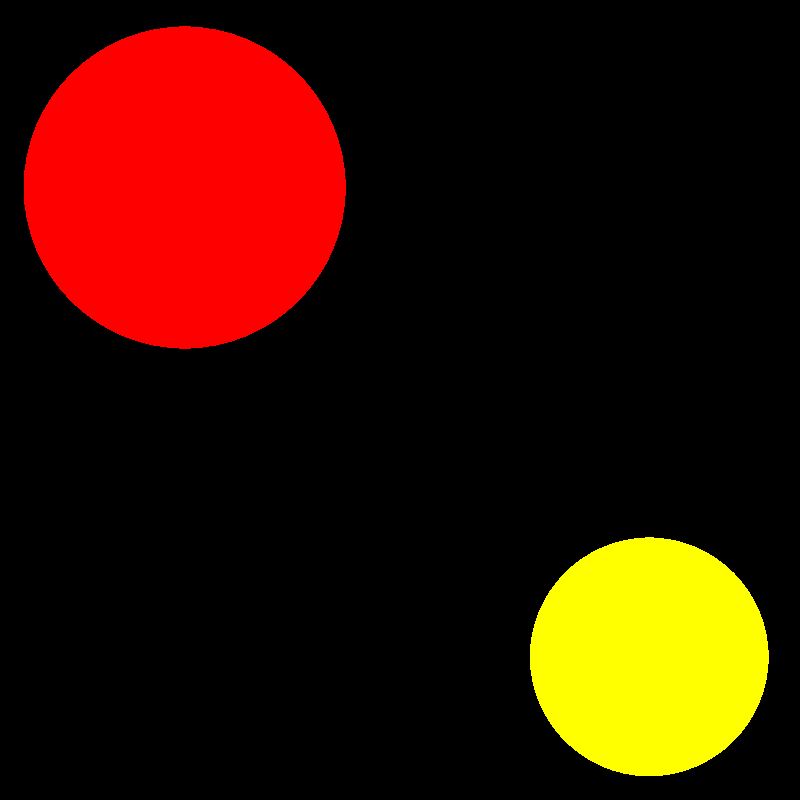
\includegraphics[width=2.5in]{imagen1.pdf}
	
	\caption{Marcas en cada robot}
	\label{fig_mar}
\end{figure}
En el sistema de vision proponemos utilizar los m\'etodos de el filtro de Gauss y la transformada de Hough. Para realizar esto utilizamos la libreria de OpenCv, la cual nos da soporte para primero aplicar un filtro de gauss para eliminar el ruido en nuestra imagen, luego convertimos nuestra imagen a la escala de grises, y finalmente aplicamos la transformada de Hough para obtener los c\'irculos en la imagen, cuyos centros tambien son hallados.\\
Una vez hallados los centros y radios de cada circulo procedemos a realizar el calculo de la ubicacion de nuestro robot, el cual utilizara unos circulos marcados como se muestra en la Fig  \ref{fig_cir}. Entonces como tenemos dos circulos de ubicacion conocida procedemos a aplicar el metodo  que nos dice que la posicion basado en esos dos circulos estara en el punto medio de la recta que une los dos centros  $c_i$ y $c_j$ de los dos circulos \cite{kelson_glo}. Entonces aplicamos punto medio entre los dos centros de los circulos:
\begin{equation}
x=\frac{x_1+y_2}{2} \qquad; y=\frac{y_1+y_2}{{2}}
\end{equation}

Una vez hallada la posicion actual del robot procedemos a hallar la orientacion con respecto al eje inicial del la imagen, de la misma forma utilizamos un metodo ya utilizado anterioremente,  el cual consiste en comparar los puntos centrales y con su tangente hallar la orientacion (angulo)\cite{kelson_glo}. El angulo $\theta$ de orientacion seria dado por:
\begin{equation}
\theta=arctan(\frac{y_1-y_2}{x_1-x_2} )
\end{equation}

\begin{figure}
\centering
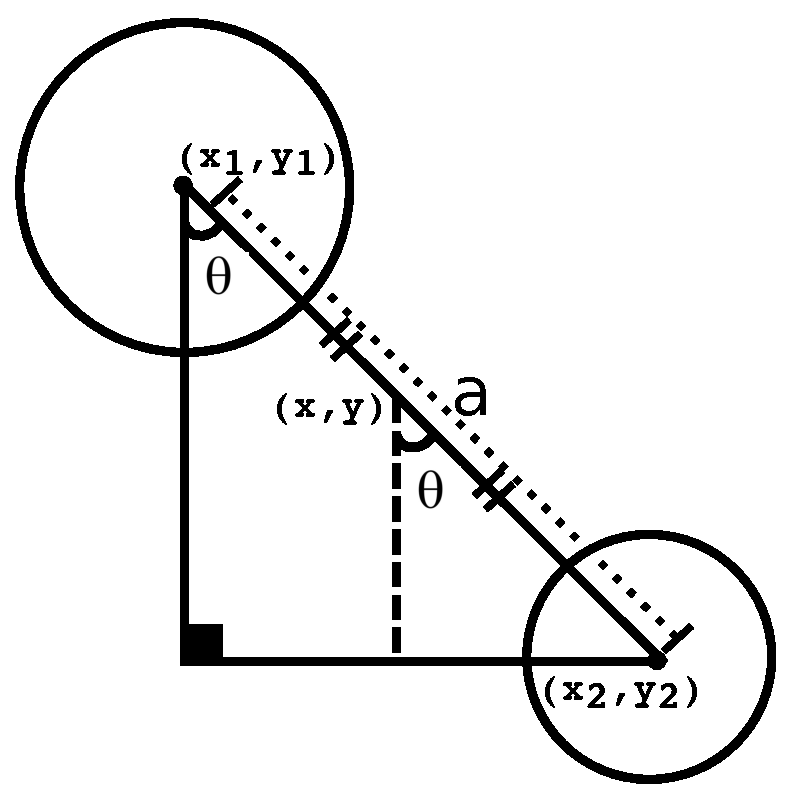
\includegraphics[width=2.5in]{imagen2.pdf}
\caption{C\'alculo de la posici\'on}
\label{fig_cir}
\end{figure}
Asi ya tenemos la posici\'on actual en cada frame y la orientaci\'on que sigue cada robot, y estamos preparados para darle estos par\'ametros a la red neuronal  y se pueda predecir su siguiente posici\'on.


\section{Seguimiento del Objeto}
Para realizar el seguimiento utilizaremos una Red Neuronal de Base Radial, la cual consiste en una red con una  capa de unidades ocultas, conectadas a las entradas y una neurona de salida, con transmicion directa (feedforward), donde las funciones de transferencia entre nodos (o neurones) son funciones simetricas radialmente. La estructura de la Red RBF es similar a la de la figura 4.4.
\begin{figure}
\centering
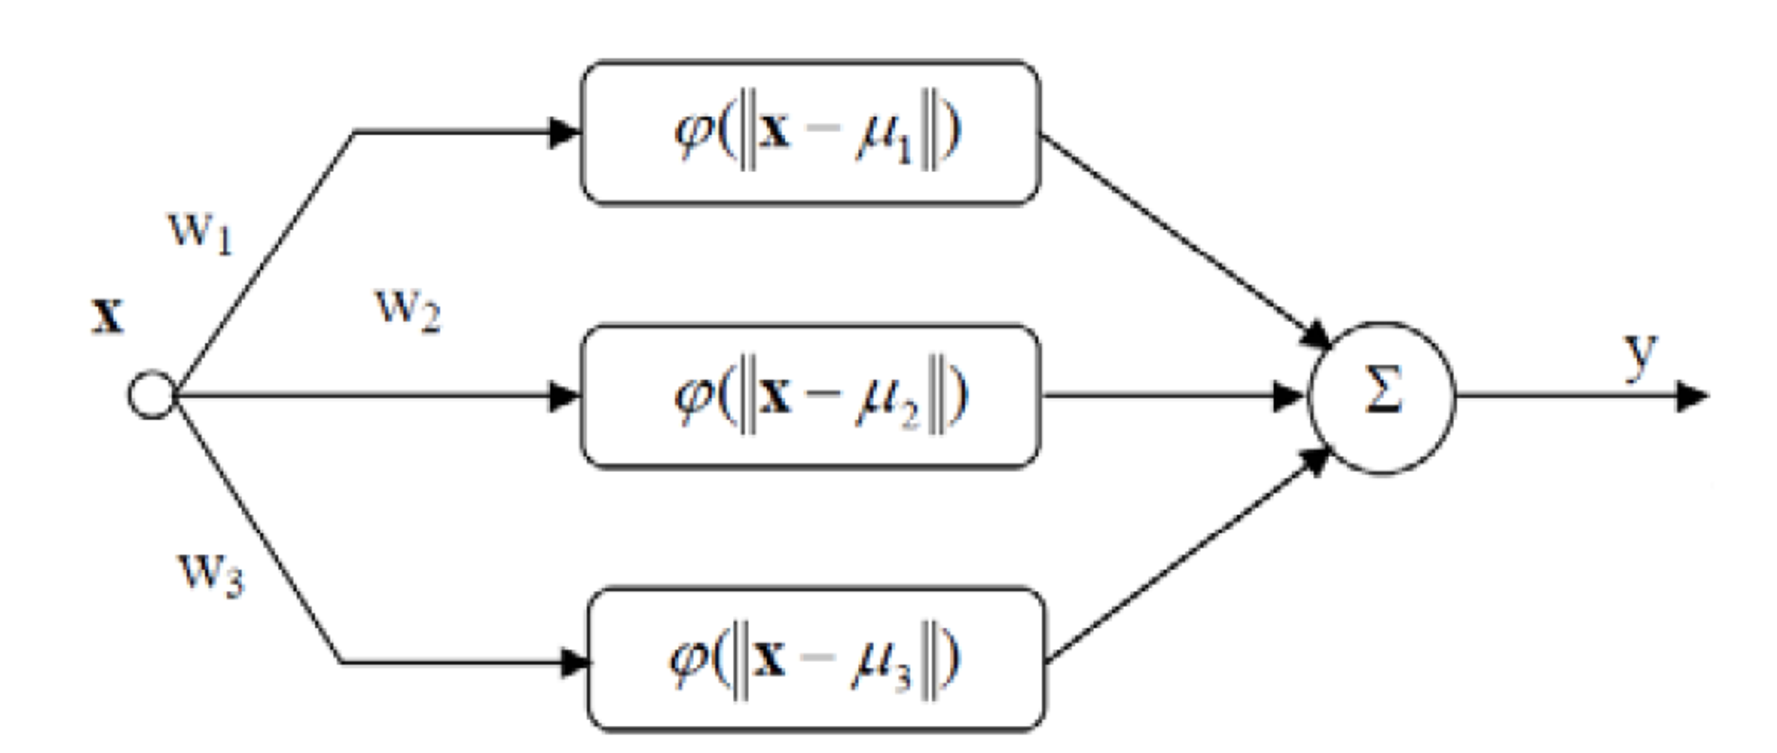
\includegraphics[width=2.5in]{RBF.pdf}
\caption{Red Neuronal de Base Radial }
\label{fig_cir}
\end{figure}

La salida para una red RBF, viene dada por: 
\[
\sum_{i=1}^{M}W_{i}\varphi(||x-\mu_i||)
\]

Donde $\varphi$ representa la funcion simetrica radialmente.
El aprendizaje en una red RBF debe ser basado en el minimizar el error, bajo la siguiente ecuacion.
\[
\sum_{p=1}^{P}(z_p-y_p)
\]
Donde $z_p$ es el valor conocido como salida, en nuestro caso la orientacion en el tiempo $t+1$, y $y_p$ es el valor de la salida de la red.\\
A esta igualdad le aplicamos el metodo de gradiente y la funcion Gaussiana,  luego de realizar los reemplazos correspondientes, nos queda que la variacion  del peso $w_i$ es como en la figura 4.5:\\
\begin{figure}
\centering
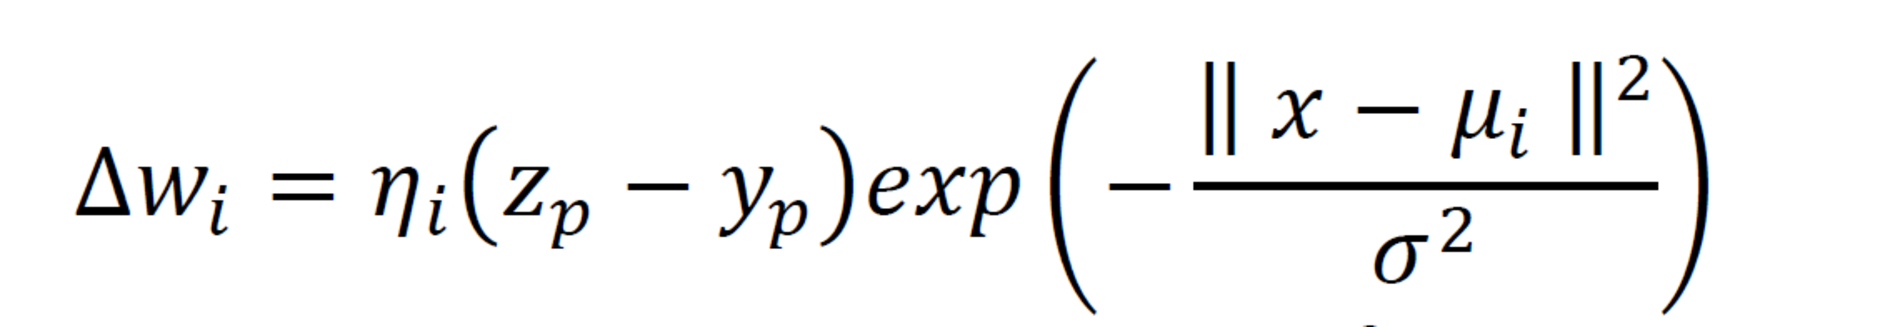
\includegraphics[width=2.5in]{eq1.pdf}
\caption{Variacion de los pesos $w_i$ }
\label{fig_cir}
\end{figure}
y para los centros quedaria como en la figura 4.6:\\
\begin{figure}
\centering
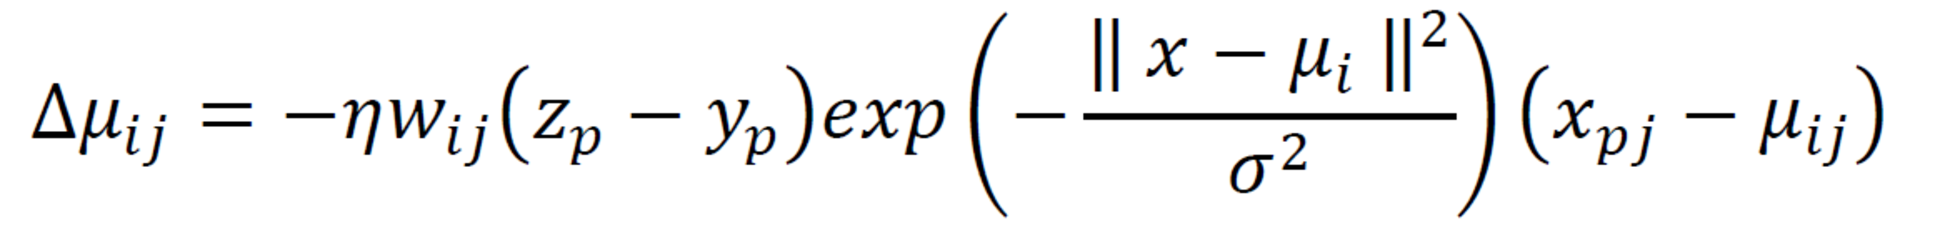
\includegraphics[width=2.5in]{eq2.pdf}
\caption{Variacion de los pesos $w_i$ }
\label{fig_cir}
\end{figure}

%
%Para este objetivo, utilizaremos el \textit{Neural Network Toolbox} de Matlab, el cual nos permite trabajar con multiples tipos de redes neuronales. En este caso hay  multiples clasificaciones de redes neuronales, las cuales pueden ser estaticas y dinamicas. Las estaticas (redes hacia adelante), no tienen retroalimentacion ni mucho menos delay(valores anteriores en el tiempo), en este tipo de redes neuronales las salidas solo dependen de la salida actual. En redes dinamic\'as la salida no solo depende de el valor actual$x_t$, sino que de valores anteriores $x_{t-1}$ , $x_{t-2}$ , $x_{t-3 }$..., de salidas anteriores, o estados en la red neuronal.\\
%Utilizaremos una red neuronal llamada \textit{Focused Time-Delay}, la cual es la red dinamica mas directa, que consiste en retroalimentaciones anteriores al actual valor. En este caso solo tendremos un neuron en nuestra red, la cual representa las orientaciones, esto porque se puede saber  hacia adonde ira el robot en el siguiente estado (resultado o salida de la red), esta red es muy util para prediccion de serie temporales (nuestro actual problema). Nuestra arquitectura es parecida a la figura 4.3:
%\begin{figure}
%\centering
%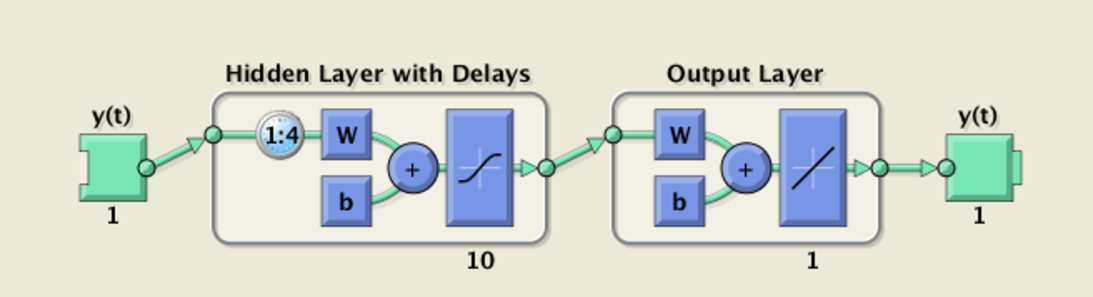
\includegraphics[width=2.5in]{red.pdf}
%\caption{Red Neuronal tipo Focused Time-Delay }
%\label{fig_cir}
%\end{figure}


%% Los cap'itulos inician con \chapter{T'itulo}, estos aparecen numerados y
%% se incluyen en el 'indice general.
%%
%% Recuerda que aqu'i ya puedes escribir acentos como: 'a, 'e, 'i, etc.
%% La letra n con tilde es: 'n.

\chapter{Evaluaci\'on}
\section{Sistema de Visi\'on}
Se ha hecho pruebas con el sistema de visi\'on el cual encuentra los c\'irculos de las marcas sobre los robots, esto es realizado con la transformada de Hough.
\begin{figure}
	\centering
	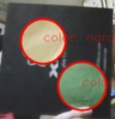
\includegraphics[width=2.5in]{imagen7.jpg}
	
	\caption{Ubicacion de los circulos}
	\label{fig_mar}
\end{figure}

Desp\'ues podemos calcular la posicion actual del robot, con los m\'etodos explicados en la propuesta.
\begin{figure}
	\centering
	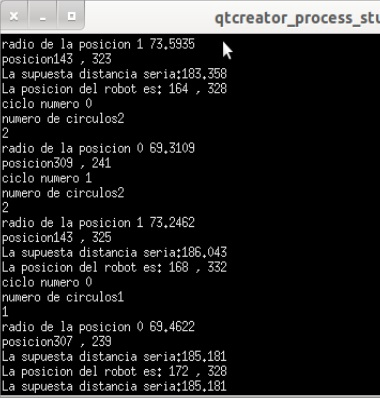
\includegraphics[width=2.5in]{imagen8.jpg}
	
	\caption{C\'alculo de la posici\'on actual del robot y la orientaci\'on}
	\label{fig_mar}
\end{figure}
%% Los cap'itulos inician con \chapter{T'itulo}, estos aparecen numerados y
%% se incluyen en el 'indice general.
%%
%% Recuerda que aqu'i ya puedes escribir acentos como: 'a, 'e, 'i, etc.
%% La letra n con tilde es: 'n.

\chapter{Conclusiones}

\begin{itemize}
\item El Sistema de Vision fue implementado utilizando la biblioteca OpenCV y se uso la IDE de programacion  QT Creator.
\item Se utilizo el \textit{Neural Network Toobox} para realizar la comparacion de nuestro algoritmo de seguimiento.
\item Para comparar se utilizo red Neuronal Dinamica la cual nos permitia utilizar valores anteriores a nuestro actual valor de entrada para tener una mejor salida, sin embargo de acuerdo a las graficas obtenidas hay mejor precision con el modelo de red RBF..
\item Las graficas obtenidas por el Matlab nos indican que nuestra red tiene un buen desempeño, ya que los datos comparados no estan muy separados entre si.
\end{itemize}
%\include{conclu}
\begin{thebibliography}{1}

\bibitem{Morales_g}
E.F.Morales and L.E. Sucar, \emph{Robots y su importancia para M\'exico}, 1st~ed.\hskip 1em plus
  0.5em minus 0.4em\relax Mexico, Instituto Nacional de Astrofisica, Optica y Electronica, Komputer Sapiens 2009 
  
\bibitem{Garcia_g}
Pablo Garcia-Robledo and Jesus Torrijos \emph{Robots de Seguridad y Defensa}\hskip 1em plus
  0.5em minus 0.4em\relax  Espa\~na, Universidad Politecnica de Madrid, 2010

\bibitem{Vasquez_g}
J.A. Garcia and L.A. Vasquez  \emph{Los Robots en el Sector Agr\'icola}\hskip 1em plus
  0.5em minus 0.4em\relax  España, Departamento  De automatica, Ingenieria Electronica e Informatica Industrial, Universidad Politecnica de Madrid,2010

\bibitem{Baltes_g}
Jacky Baltes and John Anderson \emph{Intelligent Global Vision for Teams of Mobile Robots, Mobile Robots:Perception \& Navigation, Sascha Kolski (Ed.), ISBN: 3-86611-283-1, InTech,Available from: http://www.intechopen.com/books/mobile-robots-perception-navigation/intelligent-global-vision-for-teams-of-mobile-robots}, 1st ed.\hskip 1em plus
  0.5em minus 0.4em\relax Pro Literatur Verlag, Germany/ARS Austria 2007.

\bibitem{Brezac_g}
Misel Brezac, Ivan Petrovic and Edouard Ivanjko, \emph{Robust and accurate global vision system for real time tracking of multiple mobile robots,Robotics and Autonomous Systems 56 (2008) 213-230.}\hskip 1em plus
  0.5em minus 0.4em\relax Elsiever, 2008

\bibitem{acharya_g}
Tinku Acharya and Ajoy K. Ray, \emph{Image Processing Principles and Applications, pag. 6}, 1st ed.\hskip 1em plus
  0.5em minus 0.4em\relax  B. Michaelis and G. Krell (Eds.): DAGM 2003, LNCS 2781, pp. 591–599, Springer-Verlag Berlin Heidelberg 2003.

\bibitem{kelson_glo}
Kelson Romulo Teixeira Aires, Pablo Javier Alsina, Adelardo Adelino Dantas de Medeiros , \emph{A GLOBAL VISION SYSTEM FOR MOBILE MINI-ROBOTS} ed.\hskip 1em plus 0.5em minus 0.4em\relax SIMPÓSIO BRASILEIRO DE AUTOMAÇÃO INTELIGENTE, 5, Canela, 2001

\bibitem{chabra_glo}
Manu Chhabra, Anusheel Nahar, Nishant Agrawal, Tamhant Jain,Amitabha Mukerjee, Apurva Mathad and Siddhartha Chaudhuri, \emph{Novel Approaches to Vision and Motion Control for Robot Soccer} ed.\hskip 1em plus 0.5em minus 0.4em\relax Proceedings  of the National Conference on Advance Manufacturing and Robotics, India 2004 


\bibitem{ball_glo}

Ball, David and Wyeth, Gordon and Nuske, Stephen, \emph{A global vision 
system for a robot soccer team} ed.\hskip 1em plus 0.5em minus 0.4em\relax SAustralasian Conference on Robotics and Automation, 6-8 December 2004, Canberra

\bibitem{clau_glo}
Gönner, Claudia and Rous, Martin and Kraiss, Karl-Friedrich, \emph{Real-Time Adaptive Colour Segmentation for the RoboCup Middle Size League} ed.\hskip 1em plus 0.5em minus 0.4em\relax RoboCup 2004: Robot Soccer World Cup VIII, Springer Berlin Heidelberg

 \bibitem{nummiaro_mot}
Kajta Nummiaro, Esther Koller-Meier, Tomas Svoboda, Daniel Roth, and Lucas Van Gool and Ajoy K. Ray, \emph{Color-Based Object Tracking in Multi-camera Environments}, 1st ed.\hskip 1em plus
  0.5em minus 0.4em\relax  B. Michaelis and G. Krell (Eds.): DAGM 2003, LNCS 2781, pp. 591–599, Springer-Verlag Berlin Heidelberg 2003 
  
 \bibitem{morioka_mul}
Kazuki Morioka, Silvester Kovacs, Peter Korondp, Joo-Hoo Lee and Hideki Hashimoto, \emph{Adaptative camera selection based on fuzzy automaton for object tracking in a Muticamera System} ed.\hskip 1em plus
  0.5em minus 0.4em\relax Journal of Engineering Annals of Faculty of Engineering Hunedoara, 2008 
  
 \bibitem{Dick_mot}
Anthony R. Dick and Michael J. Brooks, \emph{A Stochastic Approach to Tracking Objetcs Across Multiple  Cameras} ed.\hskip 1em plus 0.5em minus 0.4em\relax Springer -Verlag Berlin Heidelberg, 2004
 
\bibitem{garcia_mot}
Renato F. Garcia, Pedro M. Shiroma, Luiz Chaimowicz, Mario F.M. Campos, \emph{Um Arcabouco para Localizacao de Enxames de Robos} ed.\hskip 1em plus 0.5em minus 0.4em\relax Universidade Federal de Minas Gerais, Belo Horizonte,VIII Simposio Brasileiro de Automacao Inteligente, Brazil 2007

\bibitem{kumar_mot}
Piyush Kumar Rai, Kamal Tiwari, Prithwijit Guha and Amitabha Mukerjee , \emph{A cost-Effective Multiple Camera Vision System using Firewire Cameras and Software Synchronization} ed.\hskip 1em plus 0.5em minus 0.4em\relax IIT Kanpur, UP, India 2003. 

%\bibitem{karabiber_mot}
%Fethullah Karabiber,  Paolo Arena, Luigi Fortuna,  Sabestiano De Fiore,  Guido Vagliasindi and Sabri Arik , \emph{Implementation of a Moving Target Tracking Algorithm Using Eye-RIS Vision System on a Mobile Robot} ed.\hskip 1em plus 0.5em minus 0.4em\relax Springer Science+Business Media, LLC 2010 

\bibitem{hossiein_mul}
Amir Hossein Khalili and Shohreh Kasaei , \emph{Object Modeling for Multicamera Correspondence Using Fuzzy Region Color Adjacency Graphs} ed.\hskip 1em plus 0.5em minus 0.4em\relax Springer Berlin Heidelberg, Advances in Computer Science and Engineering 2009 


\bibitem{oto_mul}
Emre Oto, Frances Lau, and Hamid Aghajan , \emph{Color-Based Multiple Agent Tracking for
Wireless Image Sensor Networks} ed.\hskip 1em plus 0.5em minus 0.4em\relax Proceedings of the 8th international conference on Advanced Concepts For Intelligent Vision Systems,Springer-Verlag,2006

%\bibitem{yaldaz_mot}
%Yildiz, Alparslan and Akgul, YusufSinan , \emph{A Fast Method for Tracking People with Multiple Cameras} ed.\hskip 1em plus 0.5em minus 0.4em\relax Trends and Topics in Computer Vision,Springer Berlin Heidelberg,2012

%\bibitem{Santos_art}
%Santos, Thiago T. and Morimoto, Carlos H. , \emph{Multiple camera people detection and tracking using support integration} ed.\hskip 1em plus 0.5em minus 0.4em\relax Journal Pattern Recognition Letters,SElsevier B.V.,2011

%\bibitem{Hofman_art}
%Hofmann, M., Wolf, D., \& Rigoll, G. (2013).  \emph{Hypergraphs for Joint Multi-view Reconstruction and Multi-object Tracking}. \hskip 1em plus 0.5em minus 0.4em\relax 2013 IEEE Conference on Computer Vision and Pattern Recognition, 3650–3657. doi:10.1109/CVPR.2013.468

%\bibitem{Leal_art}
%L. Leal-Taixe, G. Pons-Moll, and B. Rosenhahn. \emph{Branch-and-price global optimization for multi-view multi-object tracking}. \hskip 1em plus 0.5em minus 0.4em\relax In 2012 IEEE Conference on Computer Vision and Pattern Recognition, June 2012
%
%\bibitem{Bilir_art}
%Bilir, S. C., \& Yemez, Y. (2012).\emph{ Non-rigid 3D shape tracking from multiview video}. \hskip 1em plus 0.5em minus 0.4em\relax  Computer Vision and Image Understanding, 116(11), 1121–1134. doi:10.1016/j.cviu.2012.07.001

%\bibitem{Greek_art}
%Tzevanidis, K., \& Argyros, A. (2011).  \emph{Unsupervised learning of background modeling parameters in multicamera systems}.  \hskip 1em plus 0.5em minus 0.4em\relax Computer Vision and Image Understanding, 115(1), 105–116. doi:10.1016/j.cviu.2010.09.003
\bibitem{lib_rob1}
Antonio Barrientos, Luis Felipe Pe\~nin, Carlos Balaguer \& Rafael Aracil (1997). \emph{Fundamentos de Rob\'otica }.  \hskip 1em plus 0.5em minus 0.4em\relax McGraw-Hill/ Interamericana Espa\~na. ISBN 84-481-0815-9

\bibitem{lib_rob2}

Bruno Siciliano, Lorenzo Sciavicco, Luigi Villani \& Giuseppe Oriolo (2009). \emph{Robotics Modelling, Plannig and Control }.  \hskip 1em plus 0.5em minus 0.4em\relax Springer-Verlag London Limited. ISBN 978-1-84628-641-4

\bibitem{art_red1}

Juan, R. Q., \& Chacón, A. (2011). \emph{Redes neuronales artificiales para el procesamiento de imágenes , una revisión de la última década}.  \hskip 1em plus 0.5em minus 0.4em\relax Revista de Infenieria Electrica, Electronica y Computacion ISSN 1870-9532
%%%aun no esta referenciada apropiadamente
%\bibitem{thrun_mot}
%Wang, C.-C., Thorpe, C., Thrun, S., Hebert, M., & Durrant-Whyte, H. (2007). \emph{Simultaneous Localization, Mapping and Moving Object Tracking}. The International Journal of Robotics Research, 26(9), 889–916. doi:10.1177/0278364907081229


\end{thebibliography}
\appendix
%% Cap'itulos incluidos despues del comando \appendix aparecen como ap'endices
%% de la tesis.
%\include{apendiceA}
%\include{apendiceB}
%\include{apendiceC}



\end{document}
